\documentclass[a4paper]{instrumentacao}

\usepackage{listings}
\usepackage{etoolbox}
\usepackage{graphicx}

\newtoggle{attachments}
\togglefalse{attachments}

\graphicspath{
	{../Resources/Images/}
	{../Resources/Mathematica/images/}
	{../Resources/MATLAB/images/}
}

%todo colocar um titulo "criativo"
\title{Sobre sensores Pt100 e NTC}
\author{Rogiel Sulzbach \and Rodrigo de Castro Silveira \and Yi Chen Wu}
\startdate{}
\finishdate{}
\emails{
	\emailaddress{R.J.S.}{rogiel@rogiel.com},
	\emailaddress{R.C.S.}{csilveira.rodrigo@gmail.com} e
	\emailaddress{Y.C.}{yichenpoa@gmail.com}
}
\resume{}
\abstract{}
\keywords{}
\institute{Universidade Federal do Rio Grande do Sul, Departamento de Engenharia Elétrica, Curso de Engenharia Elétrica, Instrumentação A, Profs. Dr. Alexandre Balbinot e Dra. Léia Bagesteiro}

\headertext{Termometria}

\begin{document}
\maketitle


\chapter{Introdução}
% ...

\chapter{Metodologia Experimental}

Nestes experimentos de laboratório foi utilizado o software Wolfram Mathematica 10.4.0 da Wolfram Research, Inc. para realizar todos os cálculos no computador utilizando precisão do tipo MachinePrecision\cite{mathematica-numerial-precision} onde a precisão dos números de ponto flutuante respeitam os critérios impostos pelo processador (64 bits) que implementam o padrão IEEE de ponto flutuante, possuem um "Épsilon de Máquina", o menor valor que somado a 1 retorna um valor diferente de 1, isto é, não causa arredondamento \cite{wikipedia-epsilon}, de $2^{-52}$, ou seja, na ordem de $10^{-16}$ e podem, portanto, serem desprezados perante a resolução de todos os outros instrumentos instrumentos utilizados no experimento. Os scripts utilizados para cálculo estão anexados ao fim do documento, na Página \pageref{ch:attachments}.

\section{Sensor de temperatura baseado em Pt100}
\label{ch:pt100}

\subsection{Calibração do sensor Pt100}
Pt100 é o nome dado à um tipo de termoresistor composto de Platina cuja variação de resistência elétrica é associada a variação de temperatura de forma linear. Outra caraterística importante é que a resistência elétrica nominal à $0ºC$ é de $100 \Omega$. Sendo um sensor linear, faz com que a criação de um termômetro eletrônico seja mais simples do que outros sensores não lineares ou de utilização mais complexa, embora a inércia térmica do sensor não permita que sejam feitas medidas em frequências elevadas como termopares permitem.

De acordo com \todo{referencia}, a função de transferência teórica do Pt100 é dada pela Equação \ref{eq:pt100}:

\begin{equation}
	R(T) \approxeq R_0 \left[1 + \alpha\left(T - T_0\right)\right]
	\label{eq:pt100}
\end{equation}

\noindent
onde $R(T)$ é a resistência elétrica em $\Omega$ do Pt100 para uma dada temperatura $T$ em $ºC$, $\alpha$ é uma constante dependente de características de construção do Pt100, $R_0$ é a resistência de referência em $\Omega$ (tipicamente $100 \Omega$ para o Pt100) e $T_0$ é a temperatura de referência em $ºC$ do termoresistor (tipicamente $0ºC$ para o Pt100).

Para estimar a função de transferência experimental do termoresistor, projetou-se um experimento onde foram feitas 2 medidas de forma aleatória para temperaturas de $18ºC$ até $78ºC$ graduadas em $2ºC$ cada. Na Figura \ref{fig:pt100-esquematico} está apresentado um desenho simplificado da configuração utilizada no experimento.

\begin{figure}[H]
\center
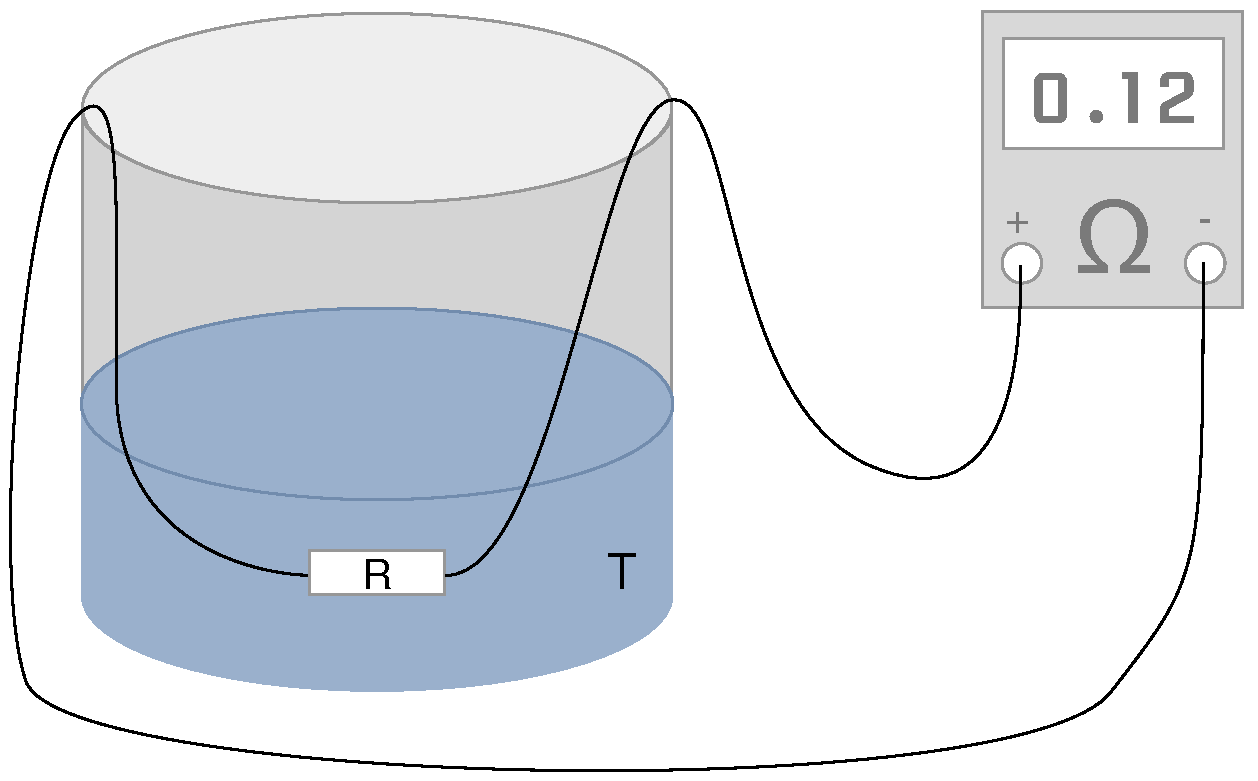
\includegraphics[width=\textwidth]{Bequer.pdf}
\caption{Desenho esquemático do experimento -- dentro de um béquer é colocada água com temperatura variando de $18ºC$ à $78ºC$ e mede-se a resistência elétrica correspondente do termoresistor.}
\label{fig:pt100-esquematico}
\end{figure}

\noindent
onde $R$ é um resistor Pt100, $T$ é a temperatura da água dentro do copo de Béquer, e o instrumento $\Omega$ é um ohmímetro.

As medidas foram feitas de forma aleatória e com 2 repetições por célula. Após a extração dos resultados, fez-se o ajuste de curvas e obteve-se a função de transferência experimental do termoresistor. Para obter a curva foi aquecida a água utilizando um aquecedor elétrico e resfriada adicionando água fria no copo de Béquer do experimento.

Com o copo de Béquer preenchido com água até a metade para que o processo de aquecimento não levasse muito tempo e nem que fosse necessário aguardar o aquecimento de um grande volume de água nem resfriar o mesmo. Uma vez que a temperatura da agua estivesse ajustada na temperatura desejada, o valor de resistência elétrica correspondente mostrado no multímetro foi anotado.

Para fazer o ajuste de temperatura da água até a temperatura de interesse foram utilizadas 2 práticas: o uso de um aquecedor elétrico para elevar a temperatura e adição de água gelada para abaixar a temperatura. Isto é, caso a temperatura de interesse estivesse acima da temperatura atual da água, um aquecedor elétrico foi utilizado para elevar a temperatura e comparar utilizando um termômetro comercial de referência e caso a temperatura de interesse estivesse abaixo da temperatura atual da água, uma pequena porção de água gelada foi adicionada ao copo até que a temperatura de desejo fosse obtida.

O termômetro comercial utilizado não possuía identificação com nome do fabricante mas informa que tem resolução de 0.1ºC dentro do intervalo de interesse com incerteza de 1ºC. Acredita-se (este fator não foi testado) que o termômetro faz uso de uma média móvel com janela entre 20 e 30 segundos devido ao tempo de resposta perceptível do termômetro durante a execução do experimento. Devido a isto, aguardava-se pelo que o valor mostrado no \textit{display} da referência estivesse, por, pelo menos, 10 segundos num valor estável.

Enquanto o aquecedor estava ligado ou logo após a adição de água gelada, com uma colher de plástico, a água era agitada para que a temperatura fosse homogeneizada por todo volume. Também foi tomado o devido cuidado para que o nem sensor nem o termômetro de referência ficassem muito próximos do aquecedor que poderia causar danos à eles ou provocar erros sistemáticos de medida devido ao super aquecimento interno nos componentes que não pudessem ser facilmente dissipados na duração do experimento.





\todo{resto do experimento do pt100}

\section{Sensor de temperatura baseado em NTC}

\subsection{Calibração do sensor NTC}
O NTC (\textit{Negative Temperatura Coefficient}) é um termoresistor, não-linear cujo coeficiente de temperatura é negativo e, portanto, sua resistência elétrica decai a medida que a temperatura se eleva.

Analogamente ao sensor de temperatura baseado em Pt100 (Página \ref{ch:pt100}), para que seja possível a construção de um termômetro utilizando um sensor do tipo NTC, é necessário que primeiramente seja levantada a função de transferência do componente para que seja possível utilizá-la na cadeia de medidas do termômetro.

De acordo com \todo{referencia}, a função de transferência teórica do NTC é dada pela Equação \ref{eq:ntc}:

\begin{equation}
	\large
	R(T) \approxeq R_0 e^{\beta\left(\frac{1}{T} - \frac{1}{T_0}\right)}
	\label{eq:ntc}
\end{equation}

\noindent
onde $R(T)$ é a resistência elétrica em $\Omega$ do NTC para uma dada temperatura $T$ em $K$, $\beta$ é uma constante dependente do material e características de construção do NTC, $R_0$ é a resistência de referência em $\Omega$ e $T_0$ é a temperatura de referência do termoresistor em $K$.

Para estimar a função de transferência experimental do NTC, projetou-se um experimento onde foram feitas 2 medidas de forma aleatória para temperaturas de $18ºC$ até $78ºC$ graduadas em $2ºC$ cada. Na Figura \ref{fig:ntc-esquematico} está apresentado um desenho simplificado da configuração utilizada no experimento.

\begin{figure}[H]
\center
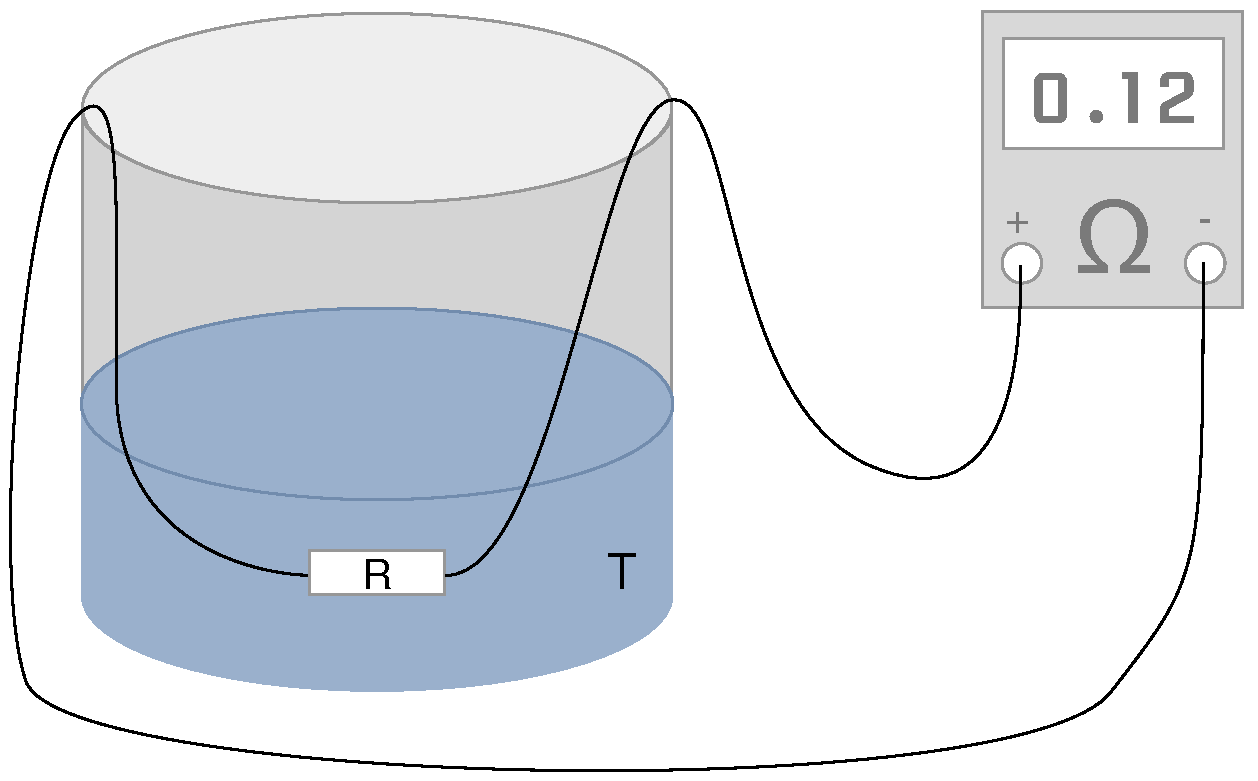
\includegraphics[width=\textwidth]{Bequer.pdf}
\caption{Desenho esquemático do experimento -- dentro de um béquer é colocada água com temperatura variando de $18ºC$ à $78ºC$ e mede-se a resistência elétrica correspondente do NTC.}
\label{fig:ntc-esquematico}
\end{figure}

\noindent
onde $R$ é um resistor NTC, $T$ é a temperatura da água dentro do copo de Béquer em $K$, e o instrumento $\Omega$ é um ohmímetro.

As medidas foram feitas de forma aleatória e com 2 repetições por célula. Após a extração dos resultados, fez-se o ajuste de curvas e obteve-se a função de transferência experimental do termoresistor.

A cadeia de medidas deste experimento é dada pela Figura \ref{fig:ntc-cadeia-medidas}:

\begin{figure}[H]
\center
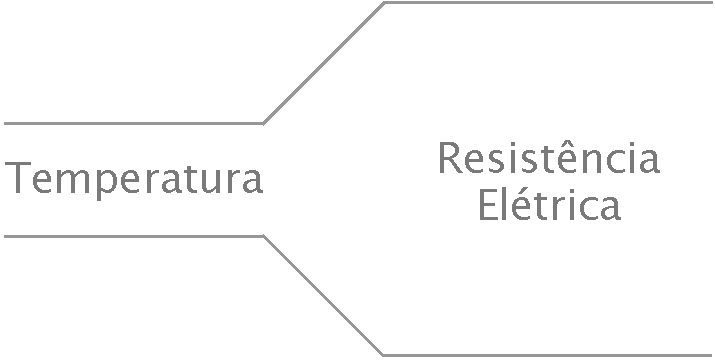
\includegraphics[width=0.7\textwidth]{CadeiaMedidas.pdf}
\caption{Cadeia de medidas para o sensor NTC}
\label{fig:ntc-cadeia-medidas}
\end{figure}

\noindent
onde a entrada é dada em temperatura (ºC) e a saída é dada em resistência elétrica ($\Omega$).

\chapter{Resultados e Discussões}

\chapter{Conclusões}


\newpage
\begin{thebibliography}{9}
\bibitem{mathematica-numerial-precision} \url{https://reference.wolfram.com/language/tutorial/NumericalPrecision.html}, acessado em 26 de abril de 2016
\bibitem{wikipedia-epsilon} \url{https://en.wikipedia.org/wiki/Machine_epsilon}, acessado em 26 de abril de 2016

\bibitem{datasheet-lm7905} Datasheet oferecido pelo fabricante do regulador de tensão LM7905PI, disponível em \url{http://www.datasheetlib.com/datasheet/190159/kia7905pi_kec-korea-electronics-corporation.html}.

\bibitem{datasheet-lm7805} Datasheet oferecido pelo fabricante do regulador de tensão LM7805CV, disponível em \url{http://www.datasheetlib.com/datasheet/221840/l7805cv_stmicroelectronics.html}.

\bibitem{datasheet-lm741} Datasheet oferecido pelo fabricante do amplificador operacional LM741, disponível em \url{http://www.datasheetlib.com/datasheet/818655/lm741_ti-texas-instruments.html}.


%\bibitem{ref1} Sobrenome, A.B.; Sobrenome, C.D. Title of the cited article. Journal Title 2007, 6, 100-110. 
%\bibitem{ref2} Balbinot, A.; Brusamarello, V.J.. Title of the cited article. Journal Title 2007, 6, 100-110. 
%\bibitem{ref3} Author, A.; Author, B. Title of the chapter. In Book Title, 2nd ed.; Editor, A., Editor, B., Eds.; Publisher: Publisher Location, Country, 2007; Volume 3, pp. 154-196.
%\bibitem{ref4} Author, A.; Author, B. Book Title, 3rd ed.; Publisher: Publisher Location, Country, 2008; 
%pp. 154-196.

\end{thebibliography}

\iftoggle{attachments}{
	\chapter*{Anexos}
	\label{ch:attachments}
	\section{Mathematica}
	\includenotebook{../Resources/Mathematica/Experimento 1-1.nb.pdf}{Pêndulo}{pendulo}
	\includenotebooksingle{../Resources/Mathematica/Incerteza potenciometro.nb}{Incerteza do potenciômetro}{incerteza-potenciometro}
	\includenotebooksingle{../Resources/Mathematica/Incertezas-Filtro.nb}{Incerteza do filtro}{incerteza-filtro}

	\section{MATLAB}
	\label{att:script-matlab}
	\lstinputlisting[
		language=MATLAB,
		numbers=left,
		caption={Script MATLAB para análise de frequência}
	]{../Resources/MATLAB/primeiro.m}
}

\end{document}
